\chapter{Case Study 5: Graphs}

\section{Introduction}

Unfortunately, information is not always convniently organised in
a tree structure. A tree structure does not make allowances for relationships
that span the tree or where cycles occur in the data. For example,
what happens when a company employee fills two roles within the company
in different departments? It would be approprate for the employee
to occur underneath both departments in the tree; the employee is
\textit{shared} between the departments or equivalently there are
two different \textit{paths} from the root of the tree to the employee.

Trees do not represent sharing and multiple paths very well. There
are strategies; for example, XML is a tree structured data format
where labels are used to mark up the elements in order to represent
sharing. When data representation requires sharing, it is usually
because the data naturally forms a \textit{graph}. Graphs can be encoded
in trees (and other forms of data representation), but if the data
requires a graph then it is probably best to use one and be done with
it.

%
\begin{figure}
\begin{center}
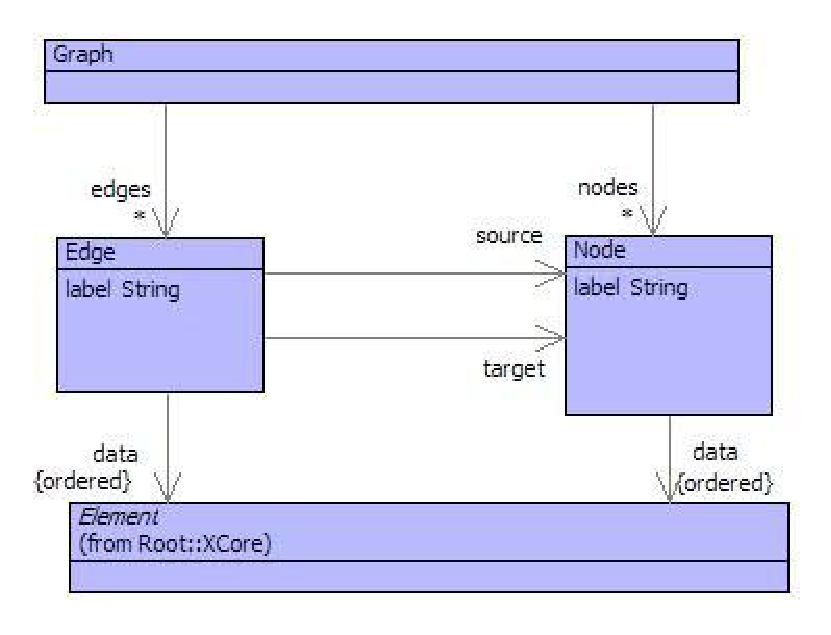
\includegraphics[scale=0.75]{CaseStudy5/figures/Graphs.pdf}

\caption{Graphs\label{fig:Graphs}}
\end{center}
\end{figure}

\section{A Model of Graphs}

Figure \ref{fig:Graphs} shows a model of graphs. A graph consists
of a set of nodes and a set of edges. Each node has a label and a
sequence of data. The label is used to identify the node and the data
is used by applications for whatever purpose they require.

Each edge has a label and data, and also has a source and target node.
Edges go between nodes and are directed. The diagram shown in figure
\ref{fig:Graphs} is itself an example of a graph where the nodes
are displayed as class boxes and the edges are shown as attribute
edges. Notice that the node labelled Element is shared (parent-wise)
between Edge and Node; equivalently there are two paths from the rot
node (labelled Graph) to the node labelled Element: Graph, Edge, Element
and Graph, Node, Element. Such sharing is difficult to represent using
trees.

Graphs are a very rich form of data representation. There is a wealth
of material written about graphs and how to process them. Here are
some useful operations on graphs defined in XOCL:

\begin{lstlisting}
context Graph
  @Operation nodeFor(label:String):Node
    @Find(node,nodes)
      when node.label() = label
      else null
    end
  end
\end{lstlisting}The operation nodeFor returns the node with the supplied label, or
null if no such node exists. The operation edgesFrom returns the set
of edges from a given node:

\begin{lstlisting}
context Graph
  @Operation edgesFrom(n:Node):Set(Edge)
    edges->select(e | e.source() = n)
  end
\end{lstlisting}Graphs are generally useful and therefore it is appropriate to have
a general purpose language construct to define a graph. As mentioned
above, each use of a graph structure will attach different amounts
of data to the nodes and labels. The data is used to support the application
specific processing of the graph. Therefore, a general purpose language
construct for graph construction should support:

\begin{enumerate}
\item Arbitrary node and edge data.
\item Plug-points for the sub-classes of Graph, Node and Edge that are used
to represent the graph.
\end{enumerate}

\section{Graph Applications}

Here are two examples of different graph applications:

\begin{lstlisting}
@Graph(Routes,Location,Road)
  London()
    M1(200) -> Leeds
    A1(50)  -> Cambridge
end

@Graph(Plan,Task,Dependency)
  Start("January")
    -> Contractors
    -> Plans
  Contractors("March")
  Plans("April")
end
\end{lstlisting}The first graph is represented as an instance of the class Routes
where the nodes and edges are instances of the classes Location and
Road. These classes are sub-classes of Graph, Node and Edge repsectively.
Locations have no data; the three locations have labels London, Leeds
and Cambridge. 

An edge is listed below the source node. In the first example graph,
there are two edges with labels M1 and A1. The edges have data 100
and 50 (being the distance in miles) and the label of the edge target
is givn after ->.

The second example is a plan graph. The nodes have data that represents
the month at which the task is completed. Edges have no labels or
data (they just represent dependencies).

The proposed structure for a graph definition has plug-points for
the graph, node and edge classes and a body consisting of a sequence
of node definitions. A node definition n is a node label, followed
by node data in parentheses followed by a series of edge definitions
for which the source of the node is n. An edge definition is an optional
edge label, optional edge data in parentheses, an arrow and then the
label of the target node. Here is an example:

\begin{lstlisting}
@Graph(G,N,E)
  n1(a,b,c)
    e1(d) -> n2
    e2() -> n3
  n2()
    e3() -> n1
  n3()
\end{lstlisting}When the parser encounters a graph definition it will synthesize program
code that, when evaluated, produces the required graph. Are there
any rules that need to be observed when this synthesis takes place?
Given the model of graphs in figure \ref{fig:Graphs}, a graph contains
nodes and edges, and edges link nodes. Here is a possible program
that produces the graph above\begin{lstlisting}
(1) let g = G()
(2) in g.addToNodes(N("n1",Seq{a,b,c}));
       g.addToNodes(N("n2"));
(3)    g.addToNodes(N("n3"));
(4)    g.addToEdges(E("e1",Seq{d},g.nodeFor("n1"),g.nodeFor("n2")));
       g.addToEdges(E("e2",g.nodeFor("n1"),g.nodeFor("n3")));
(5)    g.addToEdges(E("e3",g.nodeFor("n2"),g.nodeFor("n1")));
(6)    g
    end
\end{lstlisting}Line (1) creates the graph using the supplied class G (a sub-class
of Graph). Each node must be added first in lines (2-3) so that edges
can then be created \textit{between} the nodes in lines (4-5). Note
that the supplied classes N and E are used to create the nodes and
edges. Finally the graph is returned in line (6).

The rules for graph construction are: create the graph, add the nodes
and then add the edges. Unfortunately, the graph definition construct
does not follow this pattern; it interleaves node and edge definitions.
A strategy is required to untangle this interleaving.

One way to address the interleaving is to have the parser synthesize
an intermediate graph definition that is processes using two or more
passes. This is perfectly respectable, and often a sensible way forward
when the required processing is fairly complex. 

In this case, the processing is not that complex, so another strategy
is used. To see how this works, a few definitions are required. An
\textit{edge constructor} expects a graph and an edge class; it adds
some edges to the supplied graph. A \textit{node constructor} expects
a graph, a node class, an edge class and a collection of edge constructors;
it adds some nodes to the supplied graph and then uses the edge constructor
to add some edges.

Node definitions are synthesized into node constructors and edge definitions
into edge constructors. The trick is to build up the edge constuctors
so that they are performed after all the node constructors. Since
the edge constructors are supplied to the node constructors, this
should be easy. Using the running example from above:

\begin{lstlisting}
n3 =
  @Operation(nodeConstructor)
    @Operation(g,N,E,edgeConstructor)
      g.addToNodes(N("n3"));
      nodeConstructor(g,N,E,edgeConstructor)
    end
  end
\end{lstlisting}The node definition for n3 is transformed into an operation that is
supplied with a node constructor and returns a node constructor. This
construction allows n3 to be linked with other noe constuctors without
knowing any details -- i.e. n3 can be defined \textit{in isolation}. 

The node constructor for n2 is similar, but involves the addition
of an edge constructor:

\begin{lstlisting}
n2 =
  @Operation(nodeConstructor)
    @Operation(g,N,E,edgeConstructor)
      let e3 = 
        @Operation(g,E)
          g.addToEdges(E("e3",g.nodeFor("n2"),g.nodeFor("n1")))
        end
      in g.addToNodes(N("n2"));
         nodeConstructor(g,N,E,addEdges(edgeConstructor,e3))
      end
    end
  end
\end{lstlisting}Note how the edge constructor for e3 is added to the supplied edge
contructor (using the yet-to-be-defined addEdges) when the supplid
node constructor is activated. This is the key to deferring the construction
of edges until all the nodes have been defined.

What should addEdges do? It is used to link all the edge constructors
together so that they all get activated. It takes two edge constructors
and returns an edge constructor:

\begin{lstlisting}
@Operation addEdges(ec1,ec2)
  @Operation(g,E)
    ec1(g,E);
    ec2(g,E)
  end
end
\end{lstlisting}The noe constructor for n1 is similar, but two edge constructors are
required:

\begin{lstlisting}
n1 =
  @Operation(nodeConstructor)
    @Operation(g,N,E,edgeConstructor)
      let e1 = 
        @Operation(g,E)
          g.addToEdges(E("e1",g.nodeFor("n1")Seq{d},g.nodeFor("n2")))
        end;
          e2 = 
        @Operation(g,E)
          g.addToEdges(E("e1",g.nodeFor("n1"),g.nodeFor("n3")))
        end then
          edges = addEdges(e1,e2)
      in g.addToNodes(N("n2"));
         nodeConstructor(g,N,E,addEdges(edgeConstructor,edges))
      end
    end
  end
\end{lstlisting}The complete graph can now be defined by linking the node constructors
together and supplying a graph:

\begin{lstlisting}
let nc = addNodes(n1,addNodes(n2,addNodes(n3,noNodes)))
in nc(G(),N,E,@Operation(g,E) g end)
end
\end{lstlisting}Each of the node constructors are linked via an operation addNodes.
The left-hand argument of addNodes is an operation that maps a node
constructor to a node constructor. The right-hand argument is a node
constructor. It is easier to see how this works from the definition:

\begin{lstlisting}
@Operation addNodes(nodeCnstrCnstr,nodeCnstr2)
  @Operation(g,N,E,edgeConstructor)
    let nodeCnstr1 = nodeCnstrCnstr(nodeCnstr2)
    in nodeCnstr1(g,N,E,edgeConstructor)
    end
  end
end
\end{lstlisting}The mechanism used by addNodes is an example of a typical pattern
that threads sequences of operations together. It allows the node
constuctor encoded in nodeCnstrCnstr to occur before that encoded
in nodeCnstr2 while also allowing the edge constructors produced by
the first to be handed on to the second (because they are to be deferrred
until all the nodes are added to the graph).

There are two types of constructor, each of which can occur repeatedly
in a sequence: nodes and edges. When this occurs, it is usual to have
some way to encode an empty sequence; in this case there are noNodes
and noEdges. Both of these are constructors:

\begin{lstlisting}
@Operation noNodes(g,N,E,edgeConstuctor)
  edgeConstructor(g,E)
end

@Operation noEdges(g,E)
  null
end
\end{lstlisting}
noNodes is a node constructor that starts edge construction. Therefore,
noNodes should be the right-most node constuctor in a sequence that
is combined using addNodes. noEdges does nothing, and can occur anywhere
in a sequence.

The grammar for graph definition synthesizes node and edge constructors
combined usin addNodes and addEdge. When an empty sequence is encountered,
the gramar synthesizes noNodes and noEdges respectively. The grammar
is defined below:

\begin{lstlisting}
  @Grammar extends OCL::OCL.grammar
    Data ::= '(' es = CommaSepExps ')' { SetExp("Seq",es) }.
    Edges(s) ::= e = Edge^(s) es = Edges^(s) 
      { [| addEdges(<e>,<es>) |] } 
    | { [| noEdges |] }.
    Edge(s) ::= l = Label d = OptData '->' t = Label { [| 
      @Operation(g,E)
        g.addToEdges(E(<l>,<d>,g.nodeFor(<s>),g.nodeFor(<t>)))
      end 
    |] }.
    Graph ::= '(' mkGraph = Exp ',' mkNode = Exp ',' mkEdge = Exp')' 
      GraphBody^(mkGraph,mkNode,mkEdge).
    GraphBody(mkGraph,mkNode,mkEdge) ::= ns = Nodes 'end' { [| 
      <ns>(<mkGraph>(),<mkNode>,<mkEdge>,@Operation(g,E) g end) 
    |] }.
    Label ::= NameExp | { "".lift() }.
    NameExp ::= n = Name { n.lift() }.
    Nodes ::= n = Node ns = Nodes 
      { [| addNodes(<n>,<ns>) |] } 
    | { [| noNodes |] }.
    Node ::= l = Label d = Data e = Edges^(l) { [|
      @Operation(Cn)
        @Operation(g,N,E,Ce)
          g.addToNodes(N(<l>,<d>));
          Cn(g,N,E,addEdges(<e>,Ce))
        end
      end
    |] }.
    OptData ::= Data | { [| Seq{} |] }.
  end
\end{lstlisting}